\section[\thesection \  Training des Modells]{Training des Modells}\label{sec:training}
%
%--------------------------------------------------------------------
%

\subsection[\thesection .\thesubsection \ 
Deep Learining Computer Vision]{Deep Leaerining Computer Vision}\label{subsec:dl_cv}


% Frame 5
\begin{frame}{Convolutional Neural Networks}

    \begin{figure}
        \centering
        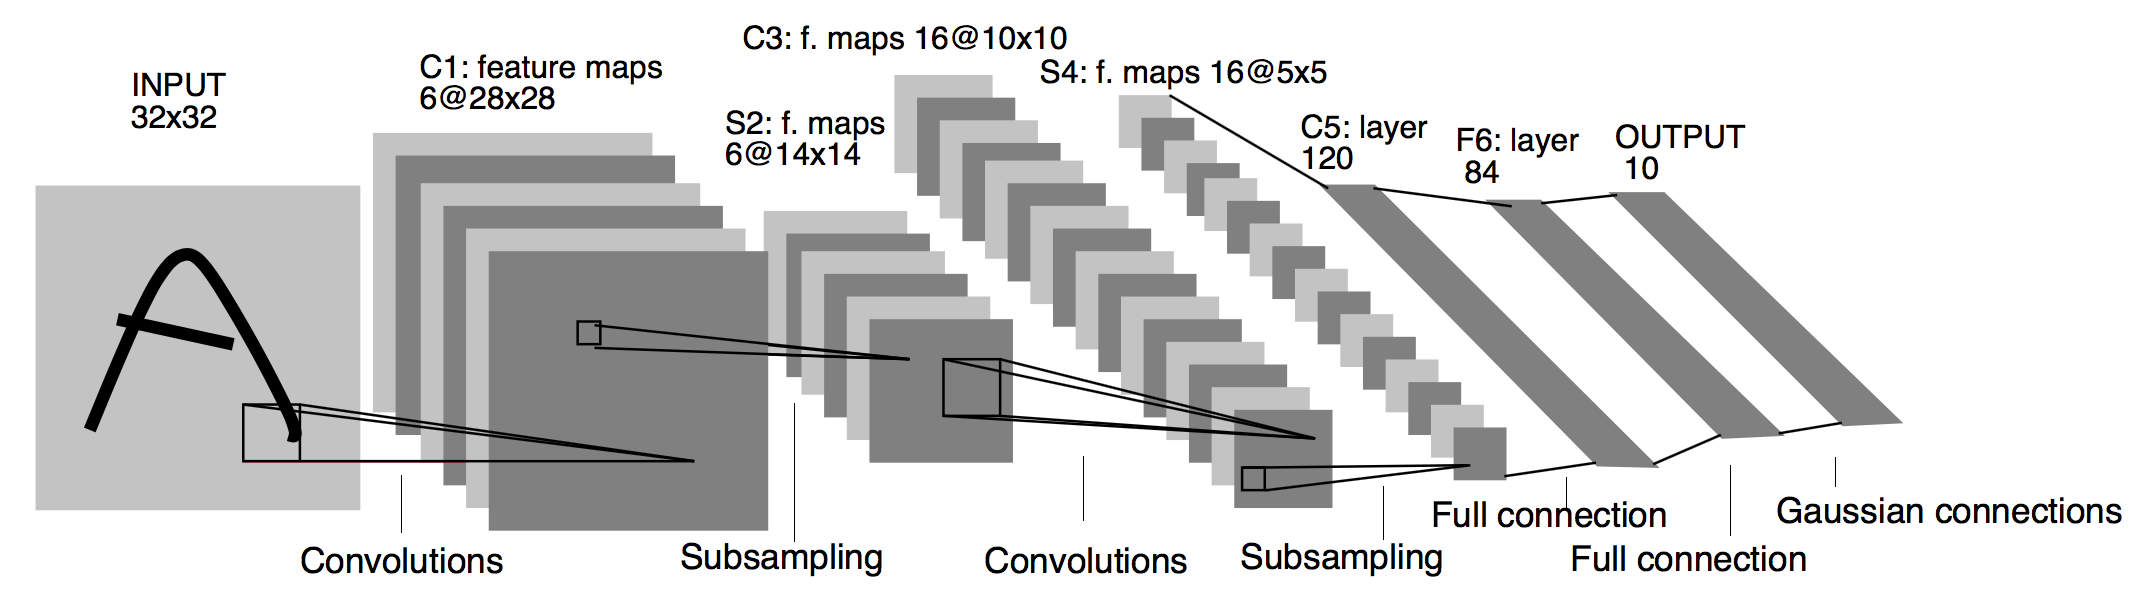
\includegraphics[width=0.7\textwidth]{Bilder/lenet.png}
    \end{figure}

    \begin{columns}[T]
        \column{0.1\columnwidth}
        \column{0.5\columnwidth}
        \begin{itemize}
            \item Convolutional Layers
            \begin{itemize}
                \item extrahieren von Features
                \item Räumliche Invarianz durch Faltung
                \item weniger Parameter durch kernel
            \end{itemize}
        \end{itemize}
        \column{0.5\columnwidth}
        \visible<2->{
        \begin{itemize}
            \item Fully Connected Layers
            \begin{itemize}
                \item Classification
            \end{itemize}
        \end{itemize}}
    \end{columns}
    \vspace{0.5cm}
    \visible<3->{
    \begin{itemize}
        \item Implementierung mithilfe Frameworks wie z.B. Tensorflow
    \end{itemize}}
        


    % \begin{block}{Arten der Erkennung}
    %     classification vs obj erk vs segmentation
    %     \\
    %     graphik
    % \end{block}
\end{frame}


% Frame 6
\begin{frame}{Objekterkennung}

    \begin{columns}[T]
        \column{0.5\columnwidth}

        \begin{itemize}
            \item zusätzliche Lokalisierung der erkannten Objekte im Bild
        \end{itemize}
        \begin{itemize}
            \item verschiedene Architekturen: 
            \begin{itemize}
                \item Regionbased CNNs (zweistufig)
                \item Single Shot Detectoren
            \end{itemize}
            verwenden beide CNNs als \textit{Backbone Networks}
        \end{itemize}

        \column{0.5\columnwidth}

        \begin{figure}
            \centering
            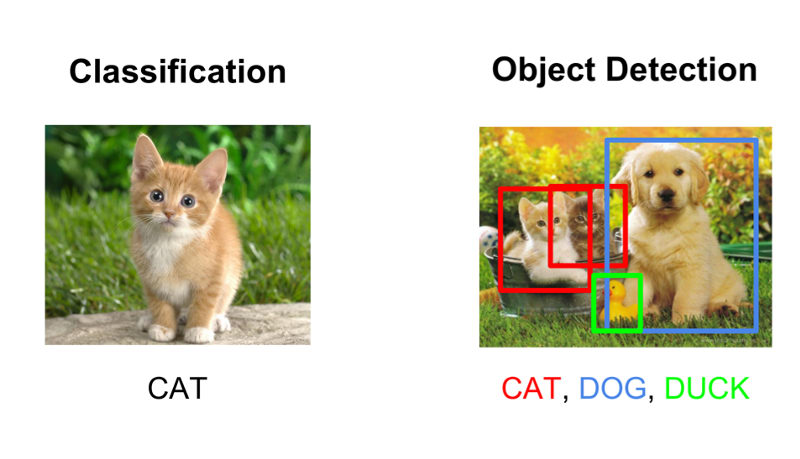
\includegraphics[width=0.9\textwidth]{Bilder/classification_detection.jpeg}
        \end{figure}
        
    \end{columns}

    \vspace{0.5cm}
        \visible<2->{
        \begin{columns}[T]
            \column{0.5\columnwidth}

            \begin{block}{Tensorflow Object Detection Api}

            \begin{itemize}
                \item Trainiert auf
                \begin{itemize}
                    \item SSD und Faster RCNN
                    \item Mobilenet, InceptionV2, Resnet50
                \end{itemize}
            \end{itemize}
        \end{block}

        \column{0.5\columnwidth}
            \begin{figure}
                \centering
                
\includegraphics[width=0.75\textwidth]{Bilder/tf_icon.png}
            \end{figure}
        \end{columns}
        }
        % rechts daneen noch grundstruktur von obj det: cnn -> 1. class, 2. regr (boxen)

\end{frame}



\subsection[\thesection .\thesubsection \ 
Sammeln und aufbereiten der Daten]{Sammeln und aufbereiten der Daten}\label{subsec:collect_data}
% Frame 7
\begin{frame}{Datensatz}
    Objekterkennung: Trainingsdaten mit Bounding Boxkoordinaten gelabelt
    \begin{block}{OpenImages}
        Frei zugängliches Datenset mit 9M Bildern
        \begin{itemize}
            \item 'Brown Bear', 'Deer' 'Fox', und weitere
        \end{itemize}
    \end{block}

    \begin{block}{Validierungs Split}
        Afteilung der Daten in:
        \begin{figure}[h]
            \centering
            \def\svgwidth{0.8\columnwidth}
            \input{Bilder/train_test_split.pdf_tex}
        \end{figure}
        Test- und Validierungs-Set dienen der Kontrolle\\
        \begin{itemize}
            \item Overfitting
        \end{itemize}
    \end{block}
\end{frame}

% Frame 8
\begin{frame}{Aufbereiten der Daten}
    \begin{block}{Augmentierung}
        \begin{itemize}
            \item Geometrisch: Verschieben, Spiegeln, Rotieren, Zoom
            \item oder: Farbwerte, Helligkeit, kontrast, Noise
        \end{itemize}
        Bild von verschiedenen Augmentierungen
    \end{block}
    \begin{block}{Graustufen}
        hier bild (von verschiedenen graustufen und helligkeiten)
    \end{block}
\end{frame}


\subsection[\thesection .\thesubsection \ 
Training]{Training}\label{subsec:train}
% Frame 9
\begin{frame}{Trainingsworkflow}
    Mit den aufbereiteten Daten und dem ausgewählten Model trainieren
    \\
    hier blockdiagramm mit [daten aufberreitung]->[model auswahl]->[trainin]->[evaluiern]->rückführung zu:
    \begin{itemize}
        \item trining: hyperparameter anpassen
        \item model: neues model auswählen
        \item date aufbereiten: andere dasten/augemntierung verwenden
    \end{itemize}
    solange bis passt
    \\
    verwendet:
    \begin{itemize}
        \item Daten: OI, mit/ohne Aug, graustufen
        \item Modelle: ssd, faster rsnn mit Backbone: Mobilenet, inception, restnet
        \item hyperparametrt \dots
    \end{itemize}
\end{frame}


\subsection[\thesection .\thesubsection \ 
Evaluierung]{Evaluierung}\label{subsec:eval}

% Frame 10
\begin{frame}{Metriken}
    Für Objekt Detection müssen 2 Faktoren berücksichtigt werden:
    \begin{itemize}
        \item existiert ein Objekt im Bild: Classificatinon
        \item wo befindet sich das obj: regression (der bbox koordinaten)
    \end{itemize}
    \begin{block}{mAP (für genauigkeit)}
        \begin{itemize}
            \item IoU > 0.5 -> True pos, else: False pos; => prec = TPs / alle Pos
            \item Recall = TPs / TPs + FN (FN falsche klasse getippt)
            \item AP = summe aller P(R) für R 0..1
            \item mAP für alle mittelwert für alle klassen
        \end{itemize}        
    \end{block}
    \begin{block}{Loss (für die Fehler rate)}
        \begin{itemize}
            \item Binärer Log Loss (CrossEntropy) für Box Classification
            \item Regressor für Box Koordinaten
        \end{itemize}
    \end{block}
\end{frame}

% frame 10
\begin{frame}{Metriken}
    Für Objekt Detection müssen 2 Faktoren berücksichtigt werden:
    \begin{itemize}
        \item existiert ein Objekt im Bild: Classificatinon
        \item wo befindet sich das obj: regression (der bbox koordinaten)
    \end{itemize}
    \begin{block}{Für die Genauigkeit}
        IoU berechnung plus graphig, ab best thresshold wird als tp gewertet, sont tn\\
        daraus ergibt sich:\\
        Precision=tp/(tp+fp)\\
        unf recall=tp/tp+fn\\
        (hier nur nicht auf bezeichnungen tp tn \dots eingehen sondern bedeutung für modell erklären)
        \\
        da mit steigendem Precision recall abnimmt, kann die fläche der Precision über recall kurve als AP (average pr) dienen 

    \end{block}
    \begin{block}{Für die Fehlerrate}
        \begin{itemize}
            \item Klassifikation: Binärer Log Loss (CrossEntropy)
            \item Regressor für Lokalisierung
        \end{itemize}
    \end{block}
\end{frame}


% Frame 11
\begin{frame}{Auswirkung von Augmentierung}

    \begin{columns}[T]
        \column{0.05\textwidth}
        \vspace{1.5cm}
        Loss\\
        \vspace{3cm}
        \visible<2->{
        mAP\\
        }

        \column{0.45\textwidth}
        \centering
        ohne Augmentierung
        \begin{figure}
            \centering
            \def\svgwidth{0.75\columnwidth}
            %\fontsize{3pt}{4pt}\selectfont
            \footnotesize
            \input{Bilder/loss_ohne_aug.pdf_tex}
            %\caption{\scriptsize ohne Augmentierung}
        \end{figure}

        \visible<2->{
        \begin{figure}
            \centering
            \def\svgwidth{0.75\columnwidth}
            \footnotesize
            \input{Bilder/mAP_ohne_aug.pdf_tex}
            %\caption{ohne Augmentierung}
        \end{figure}
        }

        \column{0.45\textwidth}
        \centering
        mit Augmentierung

        \begin{figure}
            \centering
            \def\svgwidth{0.75\columnwidth}
            \footnotesize
            \input{Bilder/loss_aug.pdf_tex}
            %\caption{ohne Augmentierung}
        \end{figure}
        \visible<2->{
        \begin{figure}
            \centering
            \def\svgwidth{0.75\columnwidth}
            \footnotesize
            \input{Bilder/mAP_aug.pdf_tex}
            %\caption{ohne Augmentierung}
        \end{figure}
        }

    \end{columns}
    \begin{itemize}
        \fontsize{7pt}{8pt}\selectfont
        \item Training: 200.000 Steps, Faster RCNN + InceptionV2, auf 9 Klassen
    \end{itemize}
\end{frame}
